\section{Introduction}

The optimisation of submerged fermentations involving filamentous microbes, which are employed in the production of a wide variety of compounds of economic importance \cite{archer2001,carlile2001,papagiannireview}, relies heavily on a knowledge of the morphology of the process micro-organism, as specific phenotypes are often associated with maximum productivity. A degree of progress has been made in elucidating correlations between fungal morphology and metabolite production in fungal fermentations and the topic has been extensively reviewed \cite{papagiannireview,wang2005,grimm2005b}. Despite such progress, significant obstacles remain in developing reproducible relationships in many cases, due to the complex architectures manifested in submerged culture.

\subsection{Morphological variation in submerged culture}

While the previous chapters of this thesis detailed work on the characterisation of mycelial growth restricted to two dimensions using membrane immobilisation, the configuration adopted by filamentous microbes often exhibits a significant three-dimensional character (Fig.~\ref{fig:SubMorph}). For example, in submerged culture, a microbe may manifest itself in the form of approximately spherical pellet structures, which may be several millimetres in diameter. Morphologically quantifying such a convoluted architecture represents a considerable challenge, particularly at the microscopic level. As a result, \lq free' hyphal elements are often targeted for microscopic analysis, as their architecture is easily confined to two dimensions (between a microscope slide and cover-slip, for example), facilitating ease of imaging.

The morphological form that results in a particular fermentation depends on environmental parameters (such as agitation speed, medium composition and pH \cite{papagiannireview}) and also on the physiology of the process microbe. For example, pellet formation can result from the aggregation of spores prior to germination, aggregation of spores and germ tubes or the aggregation of mycelia. There is evidence that conidiospores of \emph{A. oryzae} are of the agglomerative variety and tend to form aggregates as they swell, prior to germination \cite{carlsen1996a}, while the development of pellets of \emph{A. terreus} from agglomerates of spores was graphically illustrated by Bizukojc and Ledakowicz \cite{bizukojc2009}. Other organisms, such as \emph{Rhizopus nigricans}, do not agglomerate during swelling and form mycelial aggregates post-germination \cite{znidarsic1998}. Carlsen and colleagues suggested that spore agglomeration is the principle driver of pellet formation in \emph{A. oryzae} as pellets did not result when cultures were inoculated with dispersed mycelia \cite{carlsen1996a}, but other studies have since demonstrated that mycelia of \emph{A. oryzae} can agglomerate to form clumps and/or pellets \cite{amanullah2001,muller2003}.

\begin{figure}[tb]
	\centering
	\subfloat[Free element]{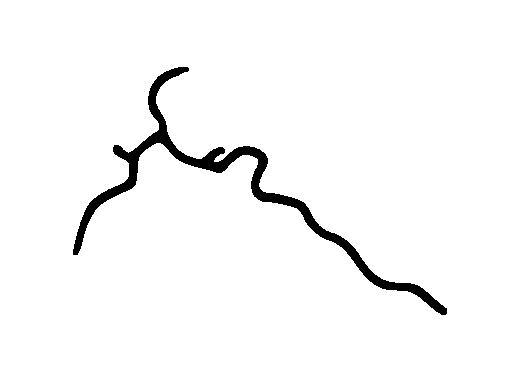
\includegraphics[width=4.5cm]{../C1/FreeHyphalElement}}
	\hspace{0.5cm}
	\subfloat[Clump]{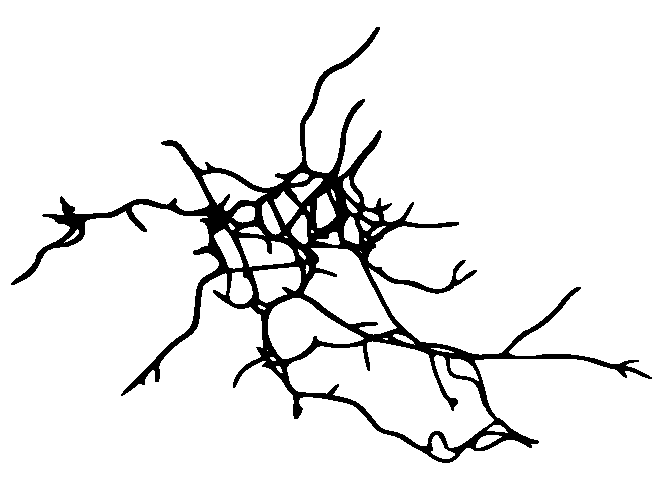
\includegraphics[width=4.5cm]{../C1/MyceliumB}}
	\hspace{0.5cm}
	\subfloat[Pellet]{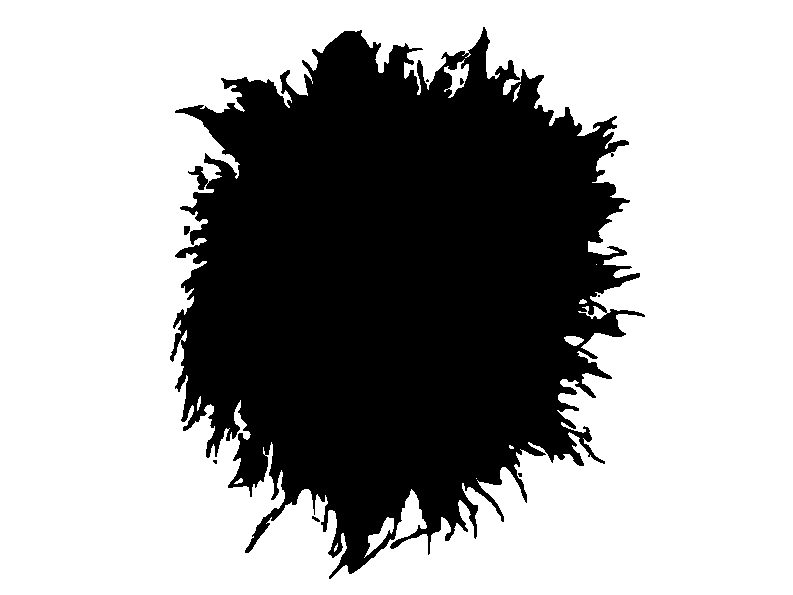
\includegraphics[width=4.5cm]{../C1/Pellet}}
	\caption{Different morphological forms adopted by filamentous microbes in submerged culture. These range from simple, branched, \lq free' hyphal structures (hyphal diameter is typically of the order of $10^{-6}$~m) to complex, composite architectures frequently termed \lq clumps'. The agglomeration of biomass can also result in the formation of dense, approximately spherical, macroscopic aggregates termed \lq pellets', which may be up to several millimetres in diameter.}
	\label{fig:SubMorph}
\end{figure}

% Diffusion limitations will eventually lead to a cessation of biomass production at the pellet core and the onset of autolysis. This eventually leads to a loss of stability and the pellet becomes more susceptible to damage by mechanical forces. Furthermore, hyphal elements at the pellet surface become weakened by aging and vacuolation, making them more susceptible to shearing. The active region within pellets and it's relationship to metabolite production has been elucidated in several studies. The diffusional limitations associated with pelleted growth would perhaps suggest that a dispersed mycelial morphology is preferable for increased product yield. However, while a pelleted morphology typically results in a broth exhibiting Newtonian properties, facilitating easier mixing, dispersed morphologies often result in non-Newtonian broth behaviour. This results in mixing problems within the bioreactor, often leading to substrate gradients and oxygen limitations, which can require substantial power inputs to overcome. 

In investigating the influence of environmental variables on microbial development, many researchers have demonstrated reproducible relationships between product yield and macro-morphology for a particular process \cite{carlsen1996a,xu2000,jppark2002,couri2003,elenshasy2006,elsabbagh2006,papagianni2006a,dobson2008a}. However, some reports have indicated that under certain conditions, product yield is seemingly independent of morphological form \cite{johansen1998,amanullah1999,papagianni1994,muller2002,amanullah2002,jayus2005}. There also exist conflicting results, such as for the production of citric acid from \emph{A. niger}. A filamentous growth form had been considered to favour maximal production \cite{paul1999} and a correlation between clump perimeter and citric acid titre derived \cite{papagianni1998}, but more recently, pelleted biomass has been suggested as optimal \cite{ali2006}. Either dispersed, filamentous growth \cite{carlsen1996a,dobson2008a,elsabbagh2006} or comparatively small, compact pellets \cite{elenshasy2006,couri2003,xu2000,jppark2002} are the most common growth forms associated with process optimisation, but occasionally, large pellets have been proposed as the preferred phenotype \cite{papagianni2006a}.

Fundamental to furthering the understanding of morphological influence on product yield is the elucidation of a relationship between hyphal branching and metabolite production, as evidence in the literature points to protein secretion occurring almost exclusively at the hyphal apex \cite{wosten1991,muller2002}. Facilitating an increase in branch formation may therefore be favourable for many processes; branching complexity has been correlated with metabolite production in \emph{A. oryzae} \cite{spohr1997,tebiesebeke2005} and  \emph{Pycnoporus cinnabarinus} \cite{jones1997}, while a swelling of hyphal tips was found to coincide with increased metabolite excretion in \emph{A. oryzae} \cite{haack2006} and \emph{A. niger} \cite{papagianni2004}. Some studies have also indicated dependencies of macro-morphological form on micro-morphological parameters and there is emerging evidence suggesting a fundamental link between kinetic parameters of growth at the microscopic level and the resultant macroscopic conformations \cite{muller2002,muller2003,eypark2006}. For example, M\"{u}ller and colleagues found that a mutant strain of \emph{A. oryzae} that exhibited a greater degree of hyphal branching (lower hyphal growth unit with respect to a wild-type strain) was less likely to form large, inseparable clumps in submerged culture \cite{muller2002}. It was also suggested that the positioning of branches (apically or sub-apically) may affect the formation and dimension of macroscopic structures. Detailed microscopic analysis is also essential to understanding development during exponential growth, an important growth phase for the production of industrial products such as biomass and growth-associated metabolites (amylases, cellulases and proteases, for example).

\subsection{Challenges associated with the morphological quantification of submerged cultures}

The complex nature of aggregates such as clumps and pellets often presents difficulties in isolating individual hyphae for the accurate quantification of branching behaviour. Furthermore, microscopic examination of composite structures such as pellets can only be performed if the size of the pellet is sufficiently small to fit within the field of view of a microscope objective lens, which is often not the case. For example, Carlsen and colleagues found that pellets of \emph{A. oryzae} grew up to 1.6~mm in diameter \cite{carlsen1996a}, while pellets of \emph{A. terreus} up to 4~mm in diameter were measured by Bizukojc and Ledakowicz \cite{bizukojc2009}. This clearly presents difficulties for conducting simultaneous assessment at the micro- and macroscopic levels when a microbe adopts such a morphology. Papagianni and Mattey used a macro-viewer connected to a CCD camera to image large pellets \cite{papagianni2004}, as did Paul and colleagues, who suspended pellets in a Petri dish filled with water, to preserve the three-dimensional architecture \cite{paul1999}. O'Cleirigh and colleagues focused exclusively on macroscopic analysis by suspending pellets of \emph{S. hygroscopicus} var. \emph{geldanus} in a Petri dish containing water and imaging with a flatbed scanner \cite{ocleirigh2003}.

Given the relatively large size of the agglomerates that can result in the submerged culturing of filamentous microbes, apparently trivial tasks such as obtaining a representative sample of biomass can prove problematic. In the case of unicellular organisms such as \emph{Saccharomyces cerevisiae}, probes have been successfully developed for \emph{in situ} culture analysis \cite{wei2007}, but such devices are not suited to the study of filamentous growth, which is not easily captured within a single focal plane. However, an automated sampling mechanism was described by Treskatis and colleagues for use in the quantification of \emph{Streptomyces tendae} T\"{u} 901/8c fermenter cultures \cite{treskatis1997}. The system performed automatic dilution and subsequent imaging (using a microscope stage-mounted chamber, similar in construction to a flow-through cell), but the analysis was restricted to macroscopic criteria ($\times 1.25$ objective), with the results consisting of classifications (rough pellets, smooth pellets, mycelial flocks, other components) assigned to biomass fractions; no morphological data beyond this was presented.

The difficulties associated with the analysis of macroscopic structures has led many researchers to focus exclusively on the dispersed growth form, using experimental arrangements such as the immobilisation of spores within a flow-through cell to study micro-morphological development in detail \cite{spohr1998,eypark2006,lubbehusen2004}. While the observations made using these simple experimental environments may be extrapolated to the more complex fermenter setting, such approaches are limited to the physiological study of a relatively small number of elements. Nonetheless, there may be potential for the utilisation of spore-immobilisation in submerged culture to provide a two-dimensional surface to support microbial growth for subsequent microscopic examination of individual elements. While such a cultivation format represents a significant deviation from conventional submerged cultivation conditions, the use of solid supports in submerged fermentations has recently been demonstrated to result in elevated metabolite production. Papagianni and Mattey found that the use of nylon supports in the cultivation of \emph{A. niger} resulted in higher citric acid production compared to a control submerged culture \cite{papagianni2004}. A beneficial effect was also reported by Bigelis and colleagues, who found that the use of polymeric membranes in liquid culture resulted in elevated metabolite production in cultures of \emph{Penicillium} sp. \emph{LL}-WF159 \cite{bigelis2006}.

\subsection{Influences on morphology}

A wide range of parameters have been utilised as a means of modifying the morphological form of filamentous microbes, including variations in medium pH \cite{hwang2004,dynesen2003}, agitation intensity \cite{papagianni1998,amanullah1999,amanullah2001,amanullah2002,rodriguezporcel2005,jppark2002,elenshasy2006} and temperature \cite{cpark2007}. Further efforts at phenotypic manipulation have involved experimentation with media composition, such as varying the nitrogen source \cite{cpark2007,nahas2002,truong2004}, phosphate source \cite{cpark2007}, the addition of metal ions \cite{couri2003,dobson2008a,kisser1980} or the modification of broth viscosity \cite{ocleirigh2005,papagianni2001}. A more invasive approach involved forcing the fermentation broth through a screen to remove pellets above a desired size \cite{shu2005}.

One of the more common means of influencing morphological variation involves modifying the type or concentration of the inoculum. A very large concentration of spores provides a large number of growth centres and a very limited amount of growth from each can result in nutrient exhaustion. Conversely, if the initial spore concentration is low, substantial growth may be required before nutrient exhaustion occurs. The distribution of biomass may thus be varied between a large number of small elements and a small number of large elements. Various reports have indicated the macroscopic impact of inoculum concentration, which is typically characterised by a decrease in mean pellet diameter for increasing initial spore concentration \cite{xu2000}. Larger increases in inoculum concentration have been demonstrated to induce completely dispersed growth in some cases \cite{papagianni2006a}. More abrupt transitions from pelleted to dispersed growth \cite{tucker1992a,jhkim2000,papagianni2006a,teng2009} have also been documented, in which inoculum effects are characterised by a sudden state change in morphology, rather than a gradual variation in one particular parameter such as projected area or pellet diameter. A microscopic response has also been described, with increasing inoculum concentration found to cause an increase in the hyphal growth unit in cultures of \emph{A. awamori} \cite{johansen1998} and \emph{A. niger} \cite{papagianni2006b}.

There is also evidence in the literature of morphological variation induced by altering the carbon source concentration in a defined medium. For example, it has been found that glucose concentration is an effective regulator of pellet size in \emph{A.~niger} \cite{papagianni2004}. At the microscopic level, it has been demonstrated that apical volume of \emph{Aspergilli} may be regulated by the surrounding glucose concentration \cite{muller2000} and further reports indicate the size and shape of mycelial clumps of \emph{A.~niger} may be influenced by glucose levels \cite{papagianni1999a}. Sub-cellular effects have also been reported, such as increased vacuolation at low substrate concentrations \cite{righelato1968,papagianni1999}, which can result in increased hyphal fragmentation.

\subsection{Chapter overview}

Having successfully applied the newly-developed image processing system (Chapter~\ref{ch:DevImagAnal}) to membrane-immobilised cultures on solid substrates (Chapter~\ref{ch:KinSolidSub}), a transition to the industry standard of submerged fermentation was now required, with a view to characterising the morphology of \emph{A. oryzae} at the microscopic level and relating microscopic form to macro-morphology and $\alpha$-amylase production (Fig.~\ref{fig:C5Overview}). The isolation of \lq free' mycelial elements was a prerequisite for the application of the imaging system, necessitating the identification of a submerged culture format in which the growth form could be reproducibly controlled.

\begin{figure}[htbp]
	\centering
	\pstool[width=(\textwidth - 1cm)]{../C5/OverviewFlowchart}{
		\psfrag{A}[Bc]{\scriptsize Aim: Relate micro-morphology}
		\psfrag{B}[Bc]{\scriptsize with macro-morphology,}
		\psfrag{C}[Bc]{\scriptsize $\alpha$-amylase production}
		\psfrag{D}[Bc]{\scriptsize Establish basic cultivation}
		\psfrag{d}[Bc]{\scriptsize conditions}
		\psfrag{E}[Bc]{\scriptsize Explore perturbations to basal}
		\psfrag{F}[Bc]{\scriptsize submerged system}
		\psfrag{G}[Bc]{\scriptsize Morphological influence of}
		\psfrag{H}[Bc]{\scriptsize carbon source variation}
		\psfrag{I}[Bc]{\scriptsize Investigate membrane-}
		\psfrag{J}[Bc]{\scriptsize immobilised culture}
		\psfrag{K}[Bc]{\scriptsize Morphological influence of}	
		\psfrag{L}[Bc]{\scriptsize inoculum concentration}
		\psfrag{M}[Bc]{\scriptsize Examine effects of detergent}
		\psfrag{N}[Bc]{\scriptsize supplementation}}
	\caption{Overview of the results presented in this chapter.}
	\label{fig:C5Overview}
\end{figure}

Initial qualitative investigations of the effect of inoculum concentration were necessary in order to determine a spore level that reproducibly resulted in the formation of a morphology suitable for image processing (such as distinct pellets), with other culture parameters (media composition, temperature) based on previously published reports. Once these basic parameters were established, the development of \emph{A. oryzae} over time in shake-flask culture could be assessed in order to establish reference points for biomass growth and $\alpha$-amylase production. Subsequently, the effect of perturbations to the basal submerged system was examined by quantifying responses to changes in the carbon source, variations in inoculum concentration and supplementation with non-ionic detergents; relationships between micro-morphology, macro-morphology and $\alpha$-amylase production were explored. In parallel with this, a novel \lq mixed-phase' culture format, consisting of immobilised biomass in submerged culture, was investigated, with a view to establishing a submerged culture format in which microscopic structures (early-stage hyphal development, in particular) could be routinely visualised.